
\chapter{Analyse van de openstaande problemen}%Lars

% Analyse van de openstaande problemen, tekorten, eventuele foute beslissingen
\section{Duratie backend API Calls}

Zoals aangehaald in sectie \ref{sec: GCE} Google Cloud Endpoints is een van de nadelen van GCE de grote variantie in duratietijd van backend API calls. Figuur \ref{fig:hist_getAllGroups} is een histogram die de relatieve frequentie weergeeft van de duratietijd van de API call getAllGroups(). (Opmerking: Gelijkaardige histrogrammen werden bekomen voor andere API calls. De histrogram is gebaseerd op 26 meetpunten verspreid over 2 dagen.) De histogram schets het probleem, nl. er is een zeer grote variatie in de data. Het gevolg hiervan is dat Triump onnatuurlijker aanvoelt. Dit is te wijten aan het feit dat een gebruiker verwacht dat eenzelfde actie steeds dezelfde duratie heeft. M.a.w. is het belangrijker dat de variantie van de duratietijd van een actie kleiner is dan de verwchtingswaarde ervan.

\begin{figure}[H]
	\centering
	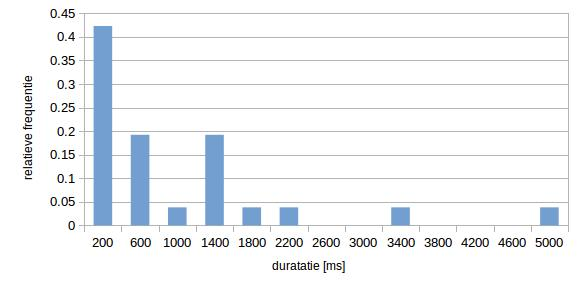
\includegraphics[scale=0.5]{prestatie_histogram_GCE}
	\caption{histogram duratietijden methode oproep getAllGroups()}
	\label{fig:hist_getAllGroups}
\end{figure}

De oplossing voor dit probleem bestaat uit caching. Wanneer een gebruiker informatie opvraagt kan onmiddelijk een lokaal opgeslagen (mogelijks verouderde) versie van het resultaat getoond worden. Eens de API call voltooid is en bijgevolg de nieuwste versie van de informatie beschikbaar is kan de verouderde versie zowel in de lokale databank als op het scherm geupdate worden. Deze oplossing wordt reeds toegepast op informatie over locatie- en overzichtelementen. Als cache of lokale databank wordt een SQLite database gebruikt. Deze database wordt aangeboden door Android. Een caching van alle data zoals de oplossing voorstelt is nog niet geïmplementeerd wegens het beperkte tijdskader van het vakoverschrijdend project.

\section{Checkin entiteiten}

In de huidige implementatie van de backend API wordt er voor iedere checkin van een gebruiker en voor iedere groep waartoe de gebruiker behoort een checkin entiteit aangemaakt. Hierdoor groeit het aantal entiteiten in de Checkin tabel zeer snel. Daarnaast komt nog dat Triump gebruik maakt van GAE Datastore voor de backend database. Bij het gebruik van deze Datastore horen quota's die beperkingen opleggen voor de grootte van de databank en voor het aantal entiteiten. 
\newline\newline
\HRule 
\newline
Hier komt een afbeelding van het percentage entiteittypes eens we wat meer data in de databank hebben \newline
\HRule
\newline\newline
% Hier moet een afbeelding komen:
% Grafiek van percentage types in datastore ...

De evidente en eenvoudigste oplossing voor dit probleem is het uitbreiden van de datastore door een dagelijks bedrag te betalen aan GAE. Een andere complexere oplossing is het opstarten van een periodieke Cron job (zie sectie ref{sec:GCE} Cron jobs) die bijvoorbeeld wekelijks de Checkin tabel 'samenvat'. De samenvatting kan gebeuren door door alle punten verzamelt door 1 groep op 1 locatie binnen een bepaalde periode toe te kennen aan 1 checkin entiteit. Op deze manier kan het aantal entiteiten drastisch beperkt worden. Nadeel van deze oplossing is het verlies aan informatie die mogelijks gebruikt kan worden voor het genereren van statistieken. 

Aangezien de opgelegde quota's m.b.t. de GAE Datastore ruimschoots voldoen en bijgevolg het probleem nog niet van toepassing is, zijn nog geen van beide oplossingen geïmplementeerd.
Indien echter het aantal gebruikers van Triump zou toenemen is het wel noodzakelijk een oplossing toe te passen.

\section{Android versies}

Android is een besturingssysteem waaraan nog vollop wordt gesleuteld door Google. Er worden met regelmaat verbeteringen en wijzigingen doorgevoerd, en dit resulteert in verschillende versies van Android.
Op \ref{fig:android_versions} kan men zien dat op het moment van schrijven voornamelijk Android versies 4.0 en later worden gebruikt. Deze zullen dan ook zeker worden ondersteunt in Triump, om een zo groot mogelijk doelpubliek te hebben. Het ondersteunen van verschillende versies brengt echter ook moeilijkheden met zich mee. Vaak worden samen met een nieuwe versie van Android, ook nieuwe concepten uitgebracht.
Een voorbeeld hiervan is de 'CardView' uit de laatste versie, Lollipop. Er is 'backward compatability' voorzien voor vorige versies van Android, maar daarop worden de 'cards' minder mooi weergegeven en zijn schaduwen niet ondersteund.
Ook is er een enorme diversiteit aan schermen van smartphones. Deze verschillen sterk in grootte en resolutie, wat ervoor zorgt dat het moeilijk is een layout te maken die op alle schermen even duidelijk en mooi overkomt.
Verder heeft Google sinds Lollipop regels opgelegd over hoe een moderne applicatie het best visueel wordt ontworpen, genaamd 'Material Design'. Het grootste probleem dat wij hiermee ondervonden was het feit dat wel werd vertelt 'wat' er moest gebeuren, maar niet 'hoe'. Details over de manier waarop de designrules moeten worden geïmplementeerd, zijn vrijwel nergens te vinden. Toch hebben we geprobeerd om ons zo goed mogelijk aan deze regels te houden.
\begin{figure}[H]
	\centering
	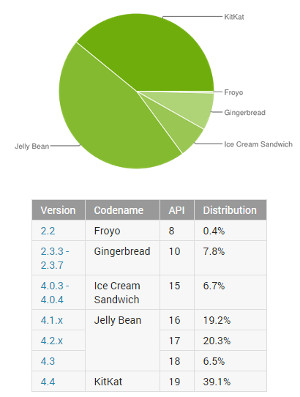
\includegraphics[scale=0.5]{android-versions}
	\caption{distributie van de Android versies in het begin van 2015}
	\label{fig:android_versions}
\end{figure}

\section{Batterijverbruik}



